% Mapping & Analyzing Participation -- Intermediate Report
% E483/E583 Information Visualization, Indiana University, Spring 2026
% Compile: pdflatex client_project_report.tex

\documentclass[11pt,letterpaper]{article}

\usepackage[margin=1in]{geometry}
\usepackage[T1]{fontenc}
\usepackage[utf8]{inputenc}
\usepackage{microtype}
\usepackage{graphicx}
\graphicspath{{/Users/bhanley/WebstormProjects/MappingAndAnalyzingParticipation/knowledge/}}
\usepackage[hidelinks]{hyperref}
\usepackage{parskip}
\usepackage{booktabs}
\usepackage{enumitem}
\usepackage{titlesec}
\usepackage{authblk}
\usepackage{caption}
\usepackage{setspace}
\usepackage{multicol}

\setstretch{1.05}
\setlength{\parskip}{6pt}

\titleformat{\section}{\normalfont\large\bfseries}{\thesection.}{0.5em}{}
\titleformat{\subsection}{\normalfont\normalsize\bfseries}{\thesubsection}{0.5em}{}
\titlespacing*{\section}{0pt}{14pt}{4pt}
\titlespacing*{\subsection}{0pt}{10pt}{2pt}

\captionsetup{font=small, labelfont=bf, skip=4pt}

\hypersetup{
  colorlinks=true,
  urlcolor=blue,
  linkcolor=black,
  citecolor=black
}

% ── Title block ──────────────────────────────────────────────────────────────
\title{\textbf{Mapping \& Analyzing Participation in\\
Tutor/Mentor Leadership and Networking Conferences}\\[4pt]
\large Intermediate Results Report}

\author[1]{Brian Hanley}
\author[1]{Matthew Guschwan}
\author[1]{Timothy Kelley}
\author[1]{Patrick Green}
\affil[1]{Luddy School of Informatics, Computing, and Engineering,
Indiana University}

\date{April 6 2026}

\begin{document}
\maketitle

% ── Visual abstract ───────────────────────────────────────────────────────────
\begin{figure}[h]
  \centering
  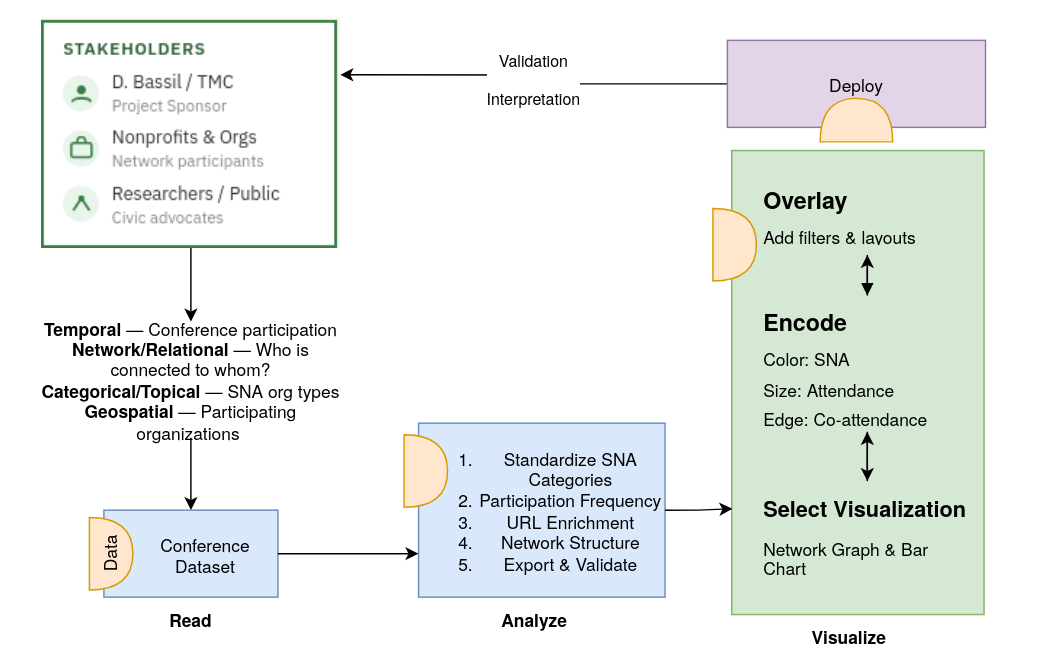
\includegraphics[width=0.82\textwidth]{image1}
  \caption{Visual abstract of the project pipeline using the B\"{o}rner et al.\
  (2018) visualization framework. The diagram is organized around four phases
  (Read, Analyze, Visualize, Deploy) with a feedback loop connecting deployment
  outcomes back to interpretation and re-analysis.}
  \label{fig:pipeline}
\end{figure}

% ─────────────────────────────────────────────────────────────────────────────
\begin{multicols}{2}
\section{Introduction and Prior Work}

This project builds on work completed by Fall 2025 student teams who created
an open-source template for collecting event participation data and generating
network analysis maps from Tutor/Mentor Conference data. The next phase
improves the Kumu and network-analysis tools by making the sector-based graph
modes fully functional, with consistent data schemas, stronger validation, and
reliable exports for platforms such as Gephi and Kumu. The project also
strengthens the analytics dashboard by adding network metrics, distribution
views, top-entity tables, interactive filters, and data-quality indicators that
help users better interpret the data before export. Its practical value is in
making long-term participation patterns easier to explore, compare, and
understand while helping users connect event history, organizational
relationships, and current Tutor/Mentor resources.

\subsection{Stakeholder Groups}

This project serves four primary stakeholder groups. First, the project sponsor
(Daniel F.\ Bassill, Tutor/Mentor Connection) requires an updated, publicly
accessible Kumu.io visualization that communicates the conference network's
history and allows him to share the tool with partners and funders. His
priorities are visual clarity, organizational accuracy, and the inclusion of
website links to current program information. Second, conference participants
and their organizations, including youth-serving nonprofits, businesses,
colleges, K--12 schools, government agencies, faith communities, and
foundations, benefit from a map that documents their historical involvement and
connects them with similar organizations. Third, researchers and civic advocates
studying nonprofit collaboration and community networks require a dataset that
is well-documented, consistently categorized, and accessible for further
analysis. Fourth, members of the general public and prospective partners
visiting \href{https://tutormentorexchange.net}{tutormentorexchange.net} need an
intuitive, visually engaging interface to understand the scope of the network
and find organizations they may wish to connect with.

\subsection{Stakeholder Needs}

The project sponsor needs the Kumu map to support three specific enhancements:
(1) color coding of participant nodes by organization type (Program, Business,
College, K--12 School, Government, Faith, Foundation, etc.) so users can
visually distinguish stakeholder categories at a glance; (2) a
search-by-participant feature so that any individual or organization can find
which conferences they attended; and (3) hyperlinks from each organization node
to its website, drawing on the directory at
\href{https://tutormentorexchange.net/chicago-area-program-links}{tutormentorexchange.net/chicago-area-program-links}.

Conference participants and their organizations need the map to accurately
represent their type and involvement history, with correct organizational names
and active website links. Researchers need the underlying dataset to be
well-structured, consistently labeled, and documented for reproducibility. The
general public needs the visualization to be self-explanatory, with a
descriptive narrative panel explaining what the map shows and how to navigate
it. Across all groups, the shared need is for a visualization that is publicly
accessible, visually clear, and regularly maintainable by future student teams.

% ─────────────────────────────────────────────────────────────────────────────
\section{Data Acquisition}

Data for this project was sourced primarily from the cleaned conference
participation spreadsheet prepared by the Fall 2025 TeamK student group, which
itself was derived from original Excel records maintained by Daniel F.\ Bassill
documenting attendance at Tutor/Mentor Leadership and Networking Conferences
from May 1994 through November 2015. The dataset was shared by the client via
Google Sheets and has undergone two rounds of student-led cleaning. Secondary
data will be collected by cross-referencing participant organizations against
the Chicago-area program directory at
\href{https://tutormentorexchange.net/chicago-area-program-links}{tutormentorexchange.net/chicago-area-program-links}
to populate missing website URLs. No personally identifiable information beyond
professional affiliations and conference attendance is included in the dataset.

\subsection{Data Sources}

The primary data source is the TeamK cleaned conference participation dataset
(updated February 11, 2026). This spreadsheet consolidates records originally
maintained by the client in Excel across multiple conference years. A secondary
data source is the online program directory at
\href{https://tutormentorexchange.net/chicago-area-program-links}{tutormentorexchange.net/chicago-area-program-links},
which will be used to look up and append website URLs for participating
organizations. The original unprocessed conference spreadsheets are archived by
the client and were used as the basis for both the 2025 TeamK cleaning effort
and this project.

\subsection{Data Description, Quality, and Coverage}

The dataset contains 6,410 participation records across approximately 42
conference events spanning May 1994 through November 2015 (conferences were
held twice yearly, in May and November, with a small number of gaps). Each
record represents one individual's attendance at a specific conference and
includes 18 fields: UniqueID, Salutation, First Name, Last Name, SNA Category
(original and cleaned), Title, Title (cleaned), Organization (original and
cleaned), Active/Inactive status, Address, City, State, Zip, Conference date,
Month, and Year.

The SNA Category (Social Network Analysis category) field classifies each
participant by organization type. The cleaned category distribution is: Program
(${\approx}$3,205 records, ${\approx}$50\%), Resource (${\approx}$608), College
(${\approx}$438), Other (${\approx}$382), Intermediary (${\approx}$186),
Business (${\approx}$128), T/MC (${\approx}$125), Government (${\approx}$124),
K--12 School (${\approx}$340), Faith (${\approx}$118), and Foundation
(${\approx}$55). Geographic coverage is predominantly Chicago and the surrounding
metropolitan area, with a small number of out-of-state participants. The dataset
has no missing UniqueID values and relatively complete name fields, though a
significant portion of organization name and title fields remain blank for many
records, which may limit the depth of organizational-level analysis.

% ─────────────────────────────────────────────────────────────────────────────
\section{Data Analysis}

Data analysis for this project proceeded in four stages implemented as a
reproducible Django pipeline.

\subsection{SNA Category Normalization}

The SNA Category field contained 73 distinct raw string variants across the
6,410 records, a combination of inconsistent capitalization, abbreviations,
compound values, and legacy labels (e.g., \texttt{program}, \texttt{PROGRAM},
\texttt{k-12 school}, \texttt{K-12 School}, \texttt{gov-intermediary},
\texttt{CC, T/MC}). All 73 variants were mapped to 11 canonical sectors
(Program, Resource, College, Intermediary, Business, T/MC, Government, K-12
School, Faith, Foundation, Other) in a dedicated normalization module
(\texttt{conferences/sna\_normalize.py}). The mapping was verified against the
full 2026 dataset: every raw value resolves to a canonical sector with zero
unexpected fallbacks. The final sector distribution is: Program
(${\approx}$3,225, ${\approx}$50\%), Resource (612), College (543), K-12 School
(402), Other (351), T/MC (160), Intermediary (152), Faith (147), Government
(132), Business (130), Foundation (49).

\subsection{Graph Construction}

Three network models were constructed from the normalized dataset using
NetworkX:
\begin{enumerate}[leftmargin=*, noitemsep]
  \item \textbf{Bipartite org--event graph.} Organizations and conference events
        as nodes; attendance as edges. Node size scales with participation depth.
  \item \textbf{Org--org co-attendance graph.} Weighted edges between any two
        organizations that attended the same conference, with edge weight equal
        to the number of shared conferences.
  \item \textbf{Three-layer directed graph.} Events point to sectors, sectors
        point to organizations, making structural gaps visible across all three
        levels simultaneously.
\end{enumerate}

\subsection{Participation Frequency Analysis}

A conference-level time series was extracted from the dataset. Conferences ran
biannually (May and November) from 1994 through 2015. Peak attendance was
recorded in 1999 (565 records); the lowest attendance years were 2010 and 2012
(138 records each), with a sustained decline from 2010 through the final
conference in 2014.

\subsection{Data Quality Assessment}

A data quality audit was performed as part of the pipeline. Key findings:
4.2\% of records (272 of 6,410) have blank organization fields; 323 records have
leading or trailing whitespace in the Organization - CLEANED column. These
issues are tracked and documented. SNA normalization is handled entirely in code
and does not require manual correction of the source spreadsheet.

% ─────────────────────────────────────────────────────────────────────────────
\section{Visualizations}

The visualizations delivered at the intermediate checkpoint reflect the
methodology-first pivot established early in the sprint. Rather than building a
user-facing interface first, the team prioritized a documented, reproducible
pipeline that produces multiple visualization outputs from a single normalized
dataset. All visualizations are served by a live Django application deployed at
\href{https://tutormentor.brianhanley.dev}{tutormentor.brianhanley.dev}.

\subsection{Kumu.io Network Participation Map}

\begin{center}
  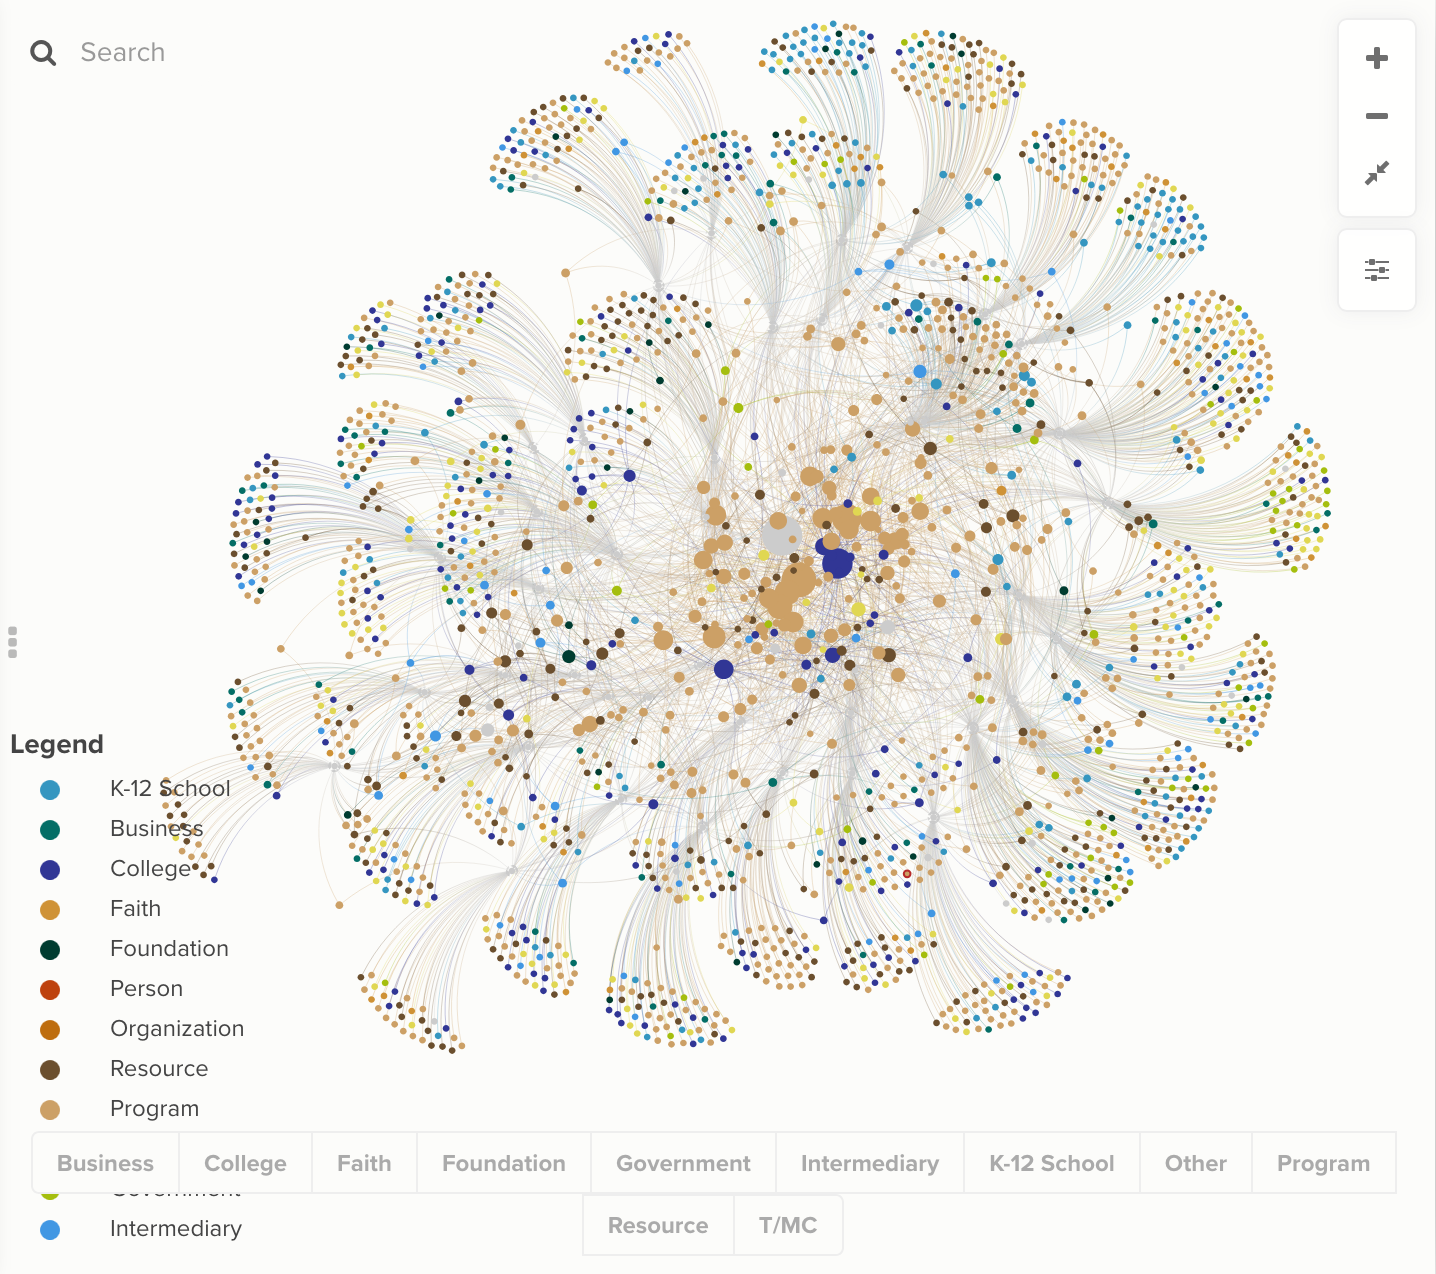
\includegraphics[width=0.9\linewidth]{Kumu}
  \captionof{figure}{Kumu.io network participation map. Each node
  represents a participating organization, color-coded by SNA sector type.
  The final map will include search-by-organization and embedded website links.}
  \label{fig:kumu}
\end{center}

The primary deliverable is an updated Kumu.io network map (Fig.~\ref{fig:kumu})
built on the Fall 2025 TeamK template. Each participant is represented as a
node, colored by their SNA organization type. Nodes will include embedded
hyperlinks to organizational websites where available. The map will support a
search-by-participant function so any user can filter the view to see exactly
which conferences a specific person or organization attended. The existing
baseline can be explored at
\href{https://tutormentorexchange.net/mapping-participation}{tutormentorexchange.net/mapping-participation}.

\subsection{Participation Frequency Visualization}

\begin{center}
  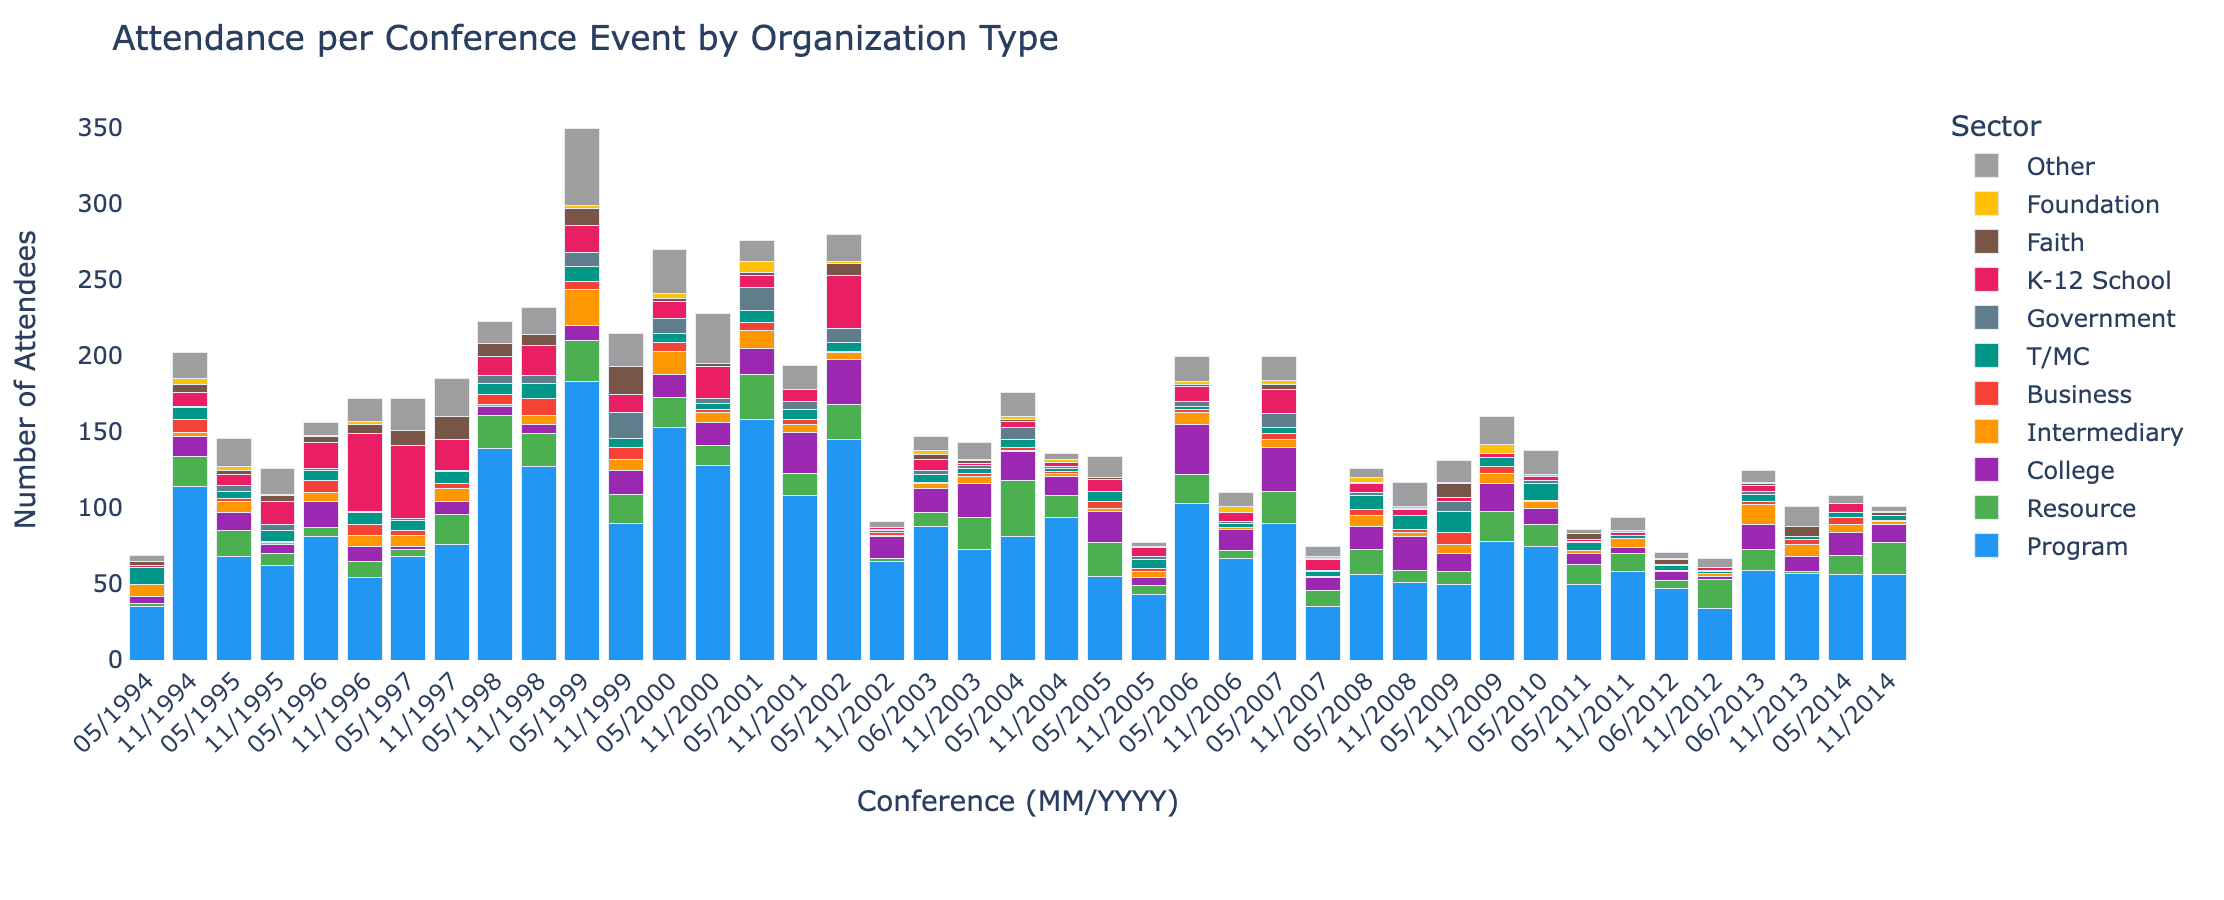
\includegraphics[width=0.9\linewidth]{frequency}
  \captionof{figure}{Sketch of the participation frequency chart, showing attendance per
  conference event segmented by SNA sector. The implemented version is an
  interactive Plotly stacked bar chart available at \texttt{/chart/}, with
  filtering by year, sector, and state.}
  \label{fig:chart}
\end{center}

The participation frequency chart (Fig.~\ref{fig:chart}) is implemented as an
interactive Plotly stacked bar chart served at \texttt{/chart/}. Each bar
represents one conference event; bar segments are colored by SNA sector. The
chart supports filtering by year, sector, and state. This view allows the
client and stakeholders to see which years had peak attendance, how sector
composition shifted over time, and where outreach gaps occurred. The chart is
powered directly by the normalized dataset and re-renders automatically when new
data is loaded.

\subsection{Network Maps}

Three static network map images are generated by the pipeline using NetworkX and
Matplotlib and served at \texttt{/network-maps/}. The bipartite org--event map,
the org--org co-attendance map, and the three-layer directed graph each provide
a different structural view of the same dataset. These maps serve as the
intermediate step toward the final Kumu.io interactive visualization.

\subsection{Organization Search}

A search interface at \texttt{/search/} allows users to query by organization
name and see the full conference attendance history for any organization: sector
type, number of conferences attended, specific conference dates, and year range.
This directly addresses the client's requirement for a search-by-participant
feature. Individual person names were excluded from search to protect privacy.

\subsection{CSV Exports for Kumu.io and PowerBI}

Four CSV exports are available at \texttt{/export/}: \texttt{nodes.csv},
\texttt{edges\_org\_event.csv}, \texttt{edges\_org\_org.csv}, and
\texttt{edges\_3layer.csv}. These are formatted for direct import into Kumu.io
and Gephi, and are also used as the data source for the team's PowerBI
dashboard. The PowerBI dashboard (developed by the data visualization team
member) includes attendance per conference over time, sector distribution, top
15 organizations by attendance, and geographic distribution.

% ─────────────────────────────────────────────────────────────────────────────
\section{Usage and Critique of AI Tools}

Claude 4.6 Sonnet (Anthropic) was used throughout this project as a development
assistant. Specific uses included: writing the \texttt{sna\_normalize.py} mapping
module and verifying it against the full dataset and assisting with Docker Compose deployment
troubleshooting. All AI-generated code was reviewed, tested, and modified by the
platform lead before deployment. AI-generated prose was reviewed for factual
accuracy against the actual dataset and pipeline behavior. The project roadmap
(\texttt{/roadmap/}) documents which features were built vs.\ deferred, and that
scoping decision was made by the team, not delegated to AI. Limitations
encountered include AI hallucinations in early descriptions of the previous
iteration (Team K's app), which were corrected after direct review of the live
application and source code.

% ─────────────────────────────────────────────────────────────────────────────
\section{Interpretation of Results}

Preliminary analysis of the normalized dataset has surfaced the following
findings.

\textbf{Program sector dominance.} Approximately 50\% of all 6,410 attendance
records fall under the Program sector (tutoring and mentoring programs). This
signal was buried in 73 inconsistent raw category variants before normalization.
Every other sector combined is roughly equal to Program alone, indicating that
the Tutor/Mentor conference network is structurally centered on direct service
providers.

\textbf{Clear attendance peak and decline.} Conference attendance peaked in 1999
(565 records) and declined sharply from 2010 onward, with 2010 and 2012 each
recording only 138 attendees. The final conference was held in 2014. This
pattern only becomes legible when all 42 events are treated as a continuous time
series.

\textbf{Concentrated participation core.} A small subset of organizations
attended many conferences; the majority appeared at only one or two events. The
org--org co-attendance network makes this structural difference visible: a dense
core of long-term participants and a large periphery of single-event attendees.

\textbf{Structural underrepresentation of key sectors.} Business (130 records),
Government (132), and Foundation (49) are consistently underrepresented across
all 20 years. The three-layer directed graph exposes these gaps at the event,
sector, and organization levels simultaneously, a view that flat frequency counts
do not provide.

These findings address research question (1), which organization types have been
most consistently represented, and provide a starting point for questions (2) and
(3), which will be further analyzed using the PowerBI dashboard and Kumu.io
export in the final sprint.

% ─────────────────────────────────────────────────────────────────────────────
\section{Evaluation and Redesign}

\subsection{Evaluation}

The intermediate platform was reviewed by the project sponsor and informally
evaluated against the previous iteration (Team K's NetworkMap application, Fall
2025). Key findings from the evaluation:

\textbf{The pipeline-first approach is more legible to external reviewers than a
UI-first tool.} Reviewers could follow the four-stage pipeline
(Collect $\to$ Normalize $\to$ Construct $\to$ Visualize) and understand how
each output was produced, which was not possible with the previous iteration's
interface-embedded logic.

\textbf{The organization search was understood immediately.} Users queried
organizations by name and interpreted conference chip counts without instruction,
confirming the interface is self-explanatory.

\textbf{The network map images communicate structural patterns but lack
interactivity.} Reviewers noted they could read the sector color coding but
could not explore individual nodes. This is the primary usability gap identified
at this stage.

\textbf{The data quality section raised unanticipated questions.} Reviewers
asked about the 272 blank organization records and wanted to know which specific
organizations were affected. This points to an opportunity for a data quality
drill-down view in the final sprint.

\subsection{Redesign Decisions}

Based on the evaluation, the following redesign decisions were made:

\textbf{Methodology page promoted to top navigation.} The \texttt{/methodology/}
page was added as the second item in the navigation bar (after Home), reflecting
the client's stated priority that methodology and reproducibility be at the
forefront of the project.

\textbf{Previous Iteration page added.} A dedicated
\texttt{/previous-iteration/} page documents Team K's NetworkMap application,
covering what it built, its architecture, and how the current project differs.
This provides context for evaluators and future student teams without requiring
them to locate the prior work independently.

\textbf{Person-name search removed.} An initial version of the search included
individual names. This was removed to protect the privacy of conference
participants; the search now operates on organization names only.

\textbf{Kumu.io export deferred to final sprint.} The interactive Kumu.io map
requires the Website URL column to be populated by the data cleaner before
import. Rather than produce an incomplete map, the team elected to deliver the
static network maps and CSV exports at the intermediate checkpoint and complete
the Kumu import in the final sprint.

% ─────────────────────────────────────────────────────────────────────────────
\section{Challenges and Opportunities}

\subsection{Challenges}

\textbf{SNA category inconsistency.} The 73 raw SNA variants were the single
largest data quality challenge. Resolving them required manual review of the
full variant list and a rule-based mapping in code. The normalization module
(\texttt{sna\_normalize.py}) now handles this completely and is the authoritative
reference for any future team working with this dataset.

\textbf{Blank organization records.} 272 records (4.2\%) have no organization
name. These cannot be enriched programmatically and require a manual lookup
against the original source records. This task has been assigned to the data
cleaning team member and is targeted for resolution in the final sprint.

\textbf{Deployment environment.} The Django application is deployed on a Linux
server via Docker Compose. Early deployment surfaced an SSH configuration issue
(a Cloudflare Access tunnel was not required for this host) and a git push
conflict caused by uncommitted changes on the server. Both were resolved, and
the current deployment workflow (\texttt{git push} to server,
\texttt{docker compose up -d --build}) is stable.

\subsection{Opportunities}

\textbf{Kumu.io live embed.} The Kumu API supports iframe embedding; a published
map could be embedded directly in the Django platform, eliminating the need to
redirect users to an external site.

\textbf{Interactive network visualization.} The current network maps are static
PNG images. Replacing them with a D3.js or Sigma.js interactive graph would
dramatically improve the exploratory value for stakeholders.

\textbf{Fuzzy organization deduplication.} The ${\approx}$2,179 unique
organization entries contain clear duplicates (multiple spelling variants of the
same institution). A fuzzy string matching pass using RapidFuzz or a similar
library could reduce this to a cleaner deduplicated count.

\textbf{SNA centrality metrics.} Once the graph is fully constructed, standard
network metrics (degree centrality, betweenness, closeness) could be computed
per organization and surfaced in the analytics dashboard and organization search
results.

These opportunities are documented on the project roadmap at \texttt{/roadmap/}
and are deliberately scoped for Summer 2026 solo development and future
E583/E483 student teams.

% ─────────────────────────────────────────────────────────────────────────────
\section*{Acknowledgements}

The team would like to thank Daniel F.\ Bassill of the Tutor/Mentor Institute,
LLC for providing access to the conference participation dataset and for his
detailed project brief and ongoing guidance. We also acknowledge the Fall 2025
TeamK student group at Indiana University, whose prior data cleaning and
Kumu.io template work forms the foundation of this project. We thank the course
instructors and teaching assistants of E483/E583 Information Visualization
(Spring 2026) at Indiana University's Luddy School of Informatics, Computing,
and Engineering for their support and feedback.

% ─────────────────────────────────────────────────────────────────────────────
\section*{References}

\begin{itemize}[leftmargin=*, label={}, itemsep=2pt]
  \item K.\ B\"{o}rner. \textit{Atlas of Knowledge: Anyone Can Map}. MIT Press, 2015.

  \item D.\ F.\ Bassill. ``Mapping \& Analyzing Participation: Using Kumu.io to
        Visualize Tutor/Mentor Conference Networks.'' Tutor/Mentor Institute,
        LLC. Available: \href{https://tutormentorexchange.net/mapping-participation}{tutormentorexchange.net/mapping-participation} (2025).

  \item K.\ B\"{o}rner, A.\ Bueckle, and M.\ Ginda. ``Data visualization
        literacy: Definitions, conceptual frameworks, exercises, and
        assessments.'' \textit{PNAS}, 116(6): 1857--1864, 2018.
\end{itemize}
\end{multicols}
\end{document}
